\Tsec{Билет №16}

\begin{leftrules}
Нелинейный показатель преломления среды; связь с кубичной нелинейностью среды. Роль стрикционного и ориентационного механизмов нелинейности.
\\ \phantom{42} \hfill \textit{лекция 10} 
\end{leftrules}





Полуклассическое описание резонансной нелинейности:
излучение – классическое, атом – квантовый.

Рассматриваем двухуровневую систему, решаем уравнение Шредингера.

Поляризация $    P = \frac{1}{2} (B e^{-i \omega t } + C) $

\begin{align}
    \frac{d B}{d t} = i \frac{d^2}{\hbar}(N_1 - N_2) - i (\omega_0 - \omega) - \frac{B}{T_2} \\
    \frac{d N_2}{d t} = - \frac{i}{4 \hbar} (BA^* - B^*A) - \frac{N_2}{T_1}
\end{align}

Искусственно добавляем времена продольной и поперечной релаксации $T_1$ и $T_2$.

Стационарное решение $\frac{d B}{d t} = 0$ даёт коэффициенты преломления и поглощения

\begin{figure}[h]
    \centering
    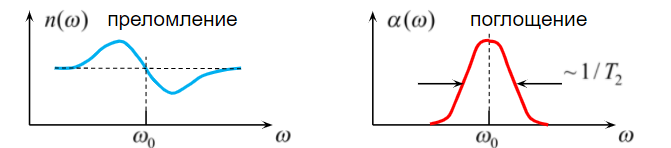
\includegraphics[width=0.6\textwidth]{figures/16-1.png}
    % \label{fig:my_label}
\end{figure}


В зависимости от длительности светового импульса возможны режимы

\begin{figure}[h]
    \centering
    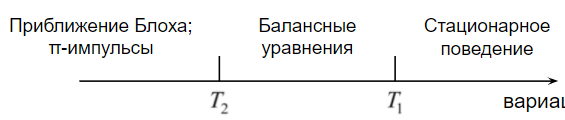
\includegraphics[width=0.5\textwidth]{figures/16-2.png}
    % \label{fig:my_label}
\end{figure}

Балансные уравнения дают сечение поглощения $\sigma(\omega)$ и

\begin{align}
    \frac{d I}{d t} = \sigma (N_2 - N_1) I \\
    \frac{d N_2}{d t } = \sigma (N_1 - N_2) \frac{I}{\hbar \omega} - \frac{N_2}{T_1}
\end{align}

В стационарном режиме $\frac{d N_2}{d t } = 0$ возникает величина интенсивности насыщения $I_{sat}$ и

\begin{equation}
    \frac{d I }{d t} = - \frac{\sigma N}{1 + \frac{I}{I_{sat}}} I
\end{equation}

Эффект просветления -- увеличение прозрачности при возрастании интенсивности падающего света
